% !TEX TS-program = pdflatex
% !TEX encoding = UTF-8 Unicode
\documentclass[xcolor={usenames,svgnames}]{beamer}

%\setbeameroption{show notes}  % frame + notes
%\setbeameroption{show only notes}  % only notes

% {{{ setup


\newcommand*{\NoENUMITEM}{} % The enumitem package disturbs Beamer.

% setup_misc.tex
% Just provide some convenient environments.
% Nothing in here should make sweeping changes to layout or the overall look.

% Place a horizontal rule.
\newcommand{\Hrule}{\hfil \rule{0.67\linewidth}{0.4pt} \hfil \\}

% Temporary note highlighting TODO.
\newcommand{\TODO}[1]{[\textbf{TODO} \textsl{#1}]}

% Just a nice way to typeset the word BibTeX.
\def\BibTeX{{\rm B\kern-.05em{\sc i\kern-.025em b}\kern-.08em
    T\kern-.1667em\lower.7ex\hbox{E}\kern-.125emX}}

\usepackage[utf8]{inputenc}

\usepackage{ifthen}

% Put pages landscape in PDF.
% http://mirror.ox.ac.uk/sites/ctan.org/macros/latex/contrib/oberdiek/pdflscape.pdf
% \begin{landscape} ... \end{landscape}
\usepackage{pdflscape}

\usepackage{grffile} % Allow dots in filenames.

\ifdefined\NoGRAPHICX \else
\usepackage{graphicx}
\graphicspath{{./}{./img/}{./shr/img/}}
\fi

% \fref and Fref for nicer references.
\usepackage[english]{babel}
\usepackage[plain]{fancyref}
\vrefwarning % NOTE: Comment and check errors before releasing documents.
\newcommand*{\fancyrefapplabelprefix}{app}
\fancyrefaddcaptions{english}{%
  \providecommand*{\frefappname}{appendix}%
  \providecommand*{\Frefappname}{Appendix}%
}
\frefformat{plain}{\fancyrefapplabelprefix}{\frefappname\fancyrefdefaultspacing#1}
\Frefformat{plain}{\fancyrefapplabelprefix}{\Frefappname\fancyrefdefaultspacing#1}
\frefformat{vario}{\fancyrefapplabelprefix}{\frefappname\fancyrefdefaultspacing#1#3}
\Frefformat{vario}{\fancyrefapplabelprefix}{\Frefappname\fancyrefdefaultspacing#1#3}

% Text Companion fonts for text symbols.
\usepackage{textcomp}

% Greek letters in text mode without changing to math mode.
\usepackage{textgreek}

% Algorithm typesetting environment.
% \begin{algorithm} ... \end{algorithm}
\usepackage{algorithmic}

\ifdefined\NoXCOLOR \else
% Lots of commands to control color.
% http://mirror.ox.ac.uk/sites/ctan.org/macros/latex/contrib/xcolor/xcolor.pdf
\usepackage[usenames,svgnames]{xcolor}
\fi

\ifdefined\NoENUMITEM \else
% Allow list customization (enumerate, itemize, description).
% http://mirror.ox.ac.uk/sites/ctan.org/macros/latex/contrib/enumitem/enumitem.pdf
\usepackage[shortlabels]{enumitem}
\fi

% Define the \FloatBarrier command.
\usepackage{placeins} % \FloatBarrier

% Extensions to the tabular environment.
% Cells which can span multiple rows.
\usepackage{multirow}
\usepackage{makecell} % \thead and other macros for table cell formatting.
\renewcommand\theadalign{bc}
\renewcommand\theadfont{\bfseries}
\renewcommand\theadgape{\Gape[4pt]}
\renewcommand\cellgape{\Gape[4pt]}
\usepackage{longtable} % Tables split over multiple pages.

\ifdefined\NoTIKZ \else
% Drawing in LaTeX.
\usepackage{tikz}
\usetikzlibrary{shapes, shapes.arrows}
\fi

\ifdefined\NoGLOSSARIES \else
% Typeset abbreviations using glossary.tex.
\usepackage{glossaries}
\makenoidxglossaries

\newglossaryentry{naiive}{
  name=na\"{\i}ve,
  description={
    is a French loanword (adjective, form of naïf) indicating having or showing
    a lack of experience, understanding or sophistication
 }
}

\newglossaryentry{ImageNet}{
  name={ImageNet},
  description={
    is an ongoing research effort to provide researchers around the world an
    easily accessible image database.
  }
}

\newglossaryentry{DutyFactor}{
  name={Duty Factor},
  description={
    Fraction of period where signal is high.
  }
}

\newacronym{ad}{AD}{Adaptive Design}
\newacronym{ai}{AI}{Artificial Intelligence}
\newacronym{amba}{AMBA}{Advanced Microcontroller Bus Architecture}
\newacronym{api}{API}{Application Prognamming Interface}
\newacronym{arm}{ARM}{Acorn RISC Machine Holdings Plc}
\newacronym{ascii}{ASCII}{American Standard Code for Information Interchange}
\newacronym{aws}{AWS}{Amazon Web Services}
\newacronym{AXI}{AXI}{Advanced/ARM eXtensible Interface}
\newacronym{ASIC}{ASIC}{Application Specific Integrated Circuit}
\newacronym{bn}{BN}{Belief Network}
\newacronym{BNN}{BNN}{Binarized Neural Network}
\newcommand{\bp}{BytePipe}
\newacronym{bpf}{BPF}{Band-Pass Filter}
\newacronym{BSC}{BSC}{Binary Symmetric Channel}
\newacronym{cam}{CAM}{Content Addressable Memory}
\newacronym{CDF}{CDF}{Cumulative Density Function}
\newacronym{CMF}{CMF}{Cumulative Mass Function}
\newacronym{cisc}{CISC}{Complex Instruction Set Computer}
\newacronym{CMOS}{CMOS}{Complementary Metal Oxide Semiconductor}
\newacronym{CNN}{CNN}{Convolutional Neural Network}
\newacronym{cpd}{CPD}{Conditional Probability Distribution}
\newacronym{CPU}{CPU}{Central Processing Unit}
\newacronym{CSV}{CSV}{Comma Separated Values}
\newacronym{CTF}{CTF}{Common Trace Format}
\newacronym{DAG}{DAG}{Directed Acyclic Graph}
\newacronym{DDR}{DDR}{Double Data Rate}
\newacronym{DFF}{DFF}{D-Type Flip-Flop}
\newacronym{DFT}{DFT}{Discrete Fourier Transform}
\newacronym{dftst}{DFT}{Design For Testability}
\newacronym{Dkl}{$D_{\text{KL}}$}{Kullback-Leibler Divergence}
\newacronym{dma}{DMA}{Direct Memory Access}
\newacronym{dsm}{\textDelta\textSigma}{Delta-Sigma Modulation}
\newacronym{DSP}{DSP}{Digital Signal Processing}
\newacronym{dtft}{DTFT}{Discrete Time Fourier Transform}
\newacronym{dvfs}{DVFS}{Dynamic Voltage and Frequency Scaling}
\newacronym{ea}{EA}{Evolutionary Algorithm}
\newacronym{eeg}{EEG}{electroencephalograph}
\newacronym{evc}{EVC}{EVent Configuration}
\newacronym{FEC}{FEC}{Forward Error Correction}
\newacronym{FFNN}{FFNN}{Feed-Forward Neural Network}
\newacronym{FFT}{FFT}{Fast Fourier Transform}
\newacronym{flit}{flit}{Flow Control Digit}
\newacronym{fifo}{FIFO}{First In First Out}
\newacronym{fmax}{$f_{\text{max}}$}{maximum operating clock frequency}
\newacronym{FSM}{FSM}{Finite State Machine}
\newacronym{ops}{Op/s}{Operations Per Second}
\newacronym{fir}{FIR}{Finite Impulse Response}
\newacronym{FOSS}{FOSS}{Free Open Source Software}
\newacronym{FPGA}{FPGA}{Field Programmable Gate Array}
\newacronym{ga}{GA}{Genetic Algorithm}
\newacronym{GPIO}{GPIO}{General Purpose Input Output}
\newacronym{HCI}{HCI}{Human-Computer Interaction}
\newacronym{hdl}{HDL}{Hardware Description Language}
\newacronym{hls}{HLS}{High Level Synthesis}
\newacronym{huels}{HLS}{Hue-Lightness-Saturation}
\newacronym{hmm}{HMM}{Hidden Markov Model}
\newacronym{hpf}{HPF}{High-Pass Filter}
\newacronym{html}{HTML}{HyperText Markup Language}
\newacronym{i2c}{I\textsuperscript{2}C}{Inter-Integrated Circuit}
\newacronym{ic}{IC}{Integrated Circuit}
\newacronym{iff}{iff}{if and only if}
\newacronym{iid}{IID}{Independent Identically Distributed}
\newacronym{iir}{IIR}{Infinite Impulse Response}
\newacronym{ip}{IP}{Intellectual Property}
%\newacronym{ip}{IP}{Internet Protocol}
\newacronym{iqr}{IQR}{Interquartile Range}
\newacronym{ISA}{ISA}{Instruction Set Architecture}
\newacronym{JTAG}{JTAG}{Joint Test Action Group}
\newacronym{KDE}{KDE}{Kernel Density Estimation}
\newacronym{mac}{MAC}{Media Access Control}
\newacronym{macc}{MAcc}{Multiply-Accumulate}
\newacronym{md}{MarkDown}{MarkDown Markup Language}
%\newacronym{md}{MD}{Medical Doctorate}
\newacronym{mesi}{MESI}{Modified/Exclusive/Shared/Invalid}
\newacronym{mimo}{MIMO}{Multiple In, Multiple Out}
\newacronym{ml}{ML}{Machine Learning}
\newacronym{mm}{MM}{Minimax}
\newacronym{mmu}{MMU}{Memory Management Unit}
\newacronym{mpnr}{Multi-PnR}{Multiple Place-and-Route}
\newacronym{msb}{MSB}{Most Significant Bit}
\newacronym{noc}{NoC}{Network-on-Chip}
\newacronym{lsb}{LSB}{Least Significant Bit}
\newacronym{lcd}{LCD}{Liquid Crystal Display}
\newacronym{LED}{LED}{Light Emitting Diode}
\newacronym{LFSR}{LFSR}{Linear Feedback Shift Register}
\newacronym{lha}{LHA}{Left Hand Associative}
\newacronym{lhs}{LHS}{Left Hand Side}
\newacronym{lpf}{LPF}{Low-Pass Filter}
\newacronym{lrm}{LRM}{Language Reference Manual}
\newacronym{LUT}{LUT}{Look Up Table}
\newacronym{lvds}{LVDS}{Low Voltage Differential Signal}
\newacronym{NN}{NN}{Neural Network}
\newacronym{obi}{OBI}{Open Bus Interface}
\newacronym{OCP}{OCP}{Open Core Protocol}
\newacronym{od}{OD}{Original Design}
\newacronym{ooo}{OoO}{Out-of-Order}
\newacronym{OS}{OS}{Operating System}
\newacronym{PCA}{PCA}{Principle Component Analysis}
\newacronym{PCB}{PCB}{Printed Circuit Board}
\newacronym{pcie}{PCIe}{PCI Express}
%\newacronym{pdf}{PDF}{Portable Document Format}
\newacronym{PDF}{PDF}{Probability Density Function}
\newacronym{PMF}{PMF}{Probability Mass Function}
\newacronym{DLL}{DLL}{Delay-Locked Loop}
\newacronym{PLL}{PLL}{Phase-Locked Loop}
\newacronym{pnr}{PnR}{Place and Route}
\newacronym{ppa}{PPA}{Power, Performance, Area}
\newacronym{pwm}{PWM}{Pulse-Width Modulation}
\newacronym{PRNG}{PRNG}{Pseudo-Random Number Generator}
\newacronym{ram}{RAM}{Random Access Memory}
\newacronym{rcg}{RCG}{Rocket Chip Generator}
\newacronym{ReLU}{ReLU}{Rectified Linear Unit}
\newacronym{rf}{RF}{Radio Frequency}
\newacronym{rgb}{RGB}{Red/Green/Blue}
\newacronym{rhs}{RHS}{Right Hand Side}
\newacronym{risc}{RISC}{Reduced Instruction Set Computer}
\newacronym{RNN}{RNN}{Recurrent Neural Network}
\newacronym{RTL}{RTL}{Register Transfer Language}
\newacronym{rv}{RISC-V}{RISC-Five}
\newacronym{sa}{SA}{Simulated Annealing}
\newacronym{sbsn}{SBSN}{Stochastic Bit-Stream Neuron}
\newacronym{sgb}{SGB}{Stochastic Gradient Boosting}
\newacronym{simd}{SIMD}{Single Instruction Multiple Data}
\newacronym{smp}{SMP}{Symmetric Multi-Processor}
\newacronym{SoC}{SoC}{System-on-Chip}
\newacronym{spi}{SPI}{Serial Peripheral Interface}
\newacronym{sql}{SQL}{Structured Query Language}
\newacronym{sv}{SV}{System Verilog}
\newacronym{sv2001}{SV2001}{System Verilog IEEE Std 1800-2001}
\newacronym{sv2005}{SV2005}{System Verilog IEEE Std 1800-2005}
\newacronym{sv2012}{SV2012}{System Verilog IEEE Std 1800-2012}
\newacronym{SVD}{SVD}{Singular Value Decomposition}
\newacronym{SVG}{SVG}{Scalable Vector Graphics}
\newacronym{svhn}{SVHN}{Street View House Numbers}
\newacronym{SVM}{SVM}{Support Vector Machine}
\newacronym{tl}{TileLink}{TileLink On-Chip Interconnect}
\newacronym{tlb}{TLB}{Translation Lookaside Buffer}
\newacronym{ts}{TS}{Time Series}
\newacronym{TUI}{TUI}{Text User Interface}
\newacronym{uarch}{\textmugreek arch}{Micro Architecture}
\newacronym{UART}{UART}{Universal Asynchronous Receiver/Transmitter}
\newacronym{UoB}{UoB}{University of Bristol}
\newacronym{URL}{URL}{Uniform Resource Locator}
\newacronym{usb}{USB}{Universal Serial Bus}
\newacronym{usbfs}{USB-FS}{USB Full Speed (12Mb/s)}
\newacronym{usbhs}{USB-HS}{USB High Speed (480Mb/s)}
\newacronym{ust}{UltraSoC}{UltraSoC Technologies Ltd}
\newacronym{Vf}{Vf}{Forward Voltage}
\newacronym{v95}{V95}{Verilog (1995)}
\newacronym{VCD}{VCD}{Value Change Dump}
\newacronym{vhdl}{VHDL}{Very High Speed Integrated Circuit Hardware Description Language}
\newacronym{vliw}{VLIW}{Very Long Instruction Word}
\newacronym{vlsi}{VLSI}{Very Large Scale Integration}
\newacronym{xml}{XML}{eXtensible Markup Language}
\newacronym{yaml}{YAML}{YAML Ain't Markup Language}

% https://en.wikipedia.org/wiki/Confusion_matrix
\newacronym{TP}{TP}{True-Positive}
\newacronym{TN}{TN}{True-Negative}
\newacronym{FP}{FP}{False-Positive}
\newacronym{FN}{FN}{False-Negative}
\newacronym{TPR}{TPR}{True Positive Rate (Sensitivity)} % Recall, Hit Rate
\newacronym{TNR}{TNR}{True Negative Rate (Specificity)} % Selectivity
\newacronym{PPV}{PPV}{Positive Predictive Value (Precision)}
\newacronym{NPV}{NPV}{Negative Predictive Value}
\newacronym{FNR}{FNR}{False Negative Rate}
\newacronym{FPR}{FPR}{False Positive Rate}
\newacronym{FDR}{FDR}{False Discovery Rate}
\newacronym{FOR}{FOR}{False Omission Rate}
\newacronym{ACC}{ACC}{Accuracy}
\newacronym{BACC}{BACC}{Balanced Accuracy}
\newacronym{MCC}{MCC}{Matthews Correlation Coefficient}
\newacronym{BMI}{BMI}{Book-Maker's Informedness}


\fi

% Captions for subfigures.
\usepackage{subcaption} % subfigure, subtable, subcaption

% Typesetting for URLs, allowing line breaks.
\usepackage{breakurl}

% Set \today to ISO format.
\usepackage{datetime}
\yyyymmdddate
\renewcommand{\dateseparator}{-}

% Add some paragraph space between lines and prefer to break a page there.
\newcommand{\blankline}{\quad\pagebreak[2]}

% Format lists with multiple columns by wrapping enumerate environment with
% \begin{multicols}{2}
%   \begin{enumerate}
%     \item foo
%     \item bar
%     \item baz
%   \end{enumerate}
% \end{multicols}
\usepackage{multicol}


% setup_math.tex
% Common math symbols.

\usepackage{amsmath,amssymb,amsfonts}
\usepackage{mathtools}
\usepackage{relsize} % mathlarger

\DeclareMathOperator{\NaN}{NaN}
\DeclarePairedDelimiter{\ceil}{\lceil}{\rceil}
\DeclarePairedDelimiter{\floor}{\lfloor}{\rfloor}
% NOTE: \! defines a negative thin space in math mode, normally 1/6 of a quad.
\newcommand{\indep}{\perp\!\!\!\!\perp} % Define the independent symbol
\newcommand{\nindep}{\centernot{\indep}} % Define the not-independent symbol
\newcommand{\nimplies}{\centernot{\implies}} % Define the not-implies symbol
\newcommand{\niff}{\centernot{\iff}} % Define the not-iff symbol
\newcommand{\Gr}{\mathcal{G}} % Graph
\newcommand{\Ed}{\mathcal{E}} % Edges
\newcommand{\Ve}{\mathcal{V}} % Nodes (vertices)
\DeclareMathOperator{\sgn}{sgn}
\newcommand{\cond}[3]{ \left( {#1} \right) \, ? \, {#2} \, : \, {#3} }

% Always use AMS font for Expectation symbol, fourier looks wrong.
\DeclareMathSymbol{\Expectation}{\mathrel}{AMSb}{"45}
\DeclareMathOperator{\Ex}{\Expectation} % Expectation
\newcommand{\sEx}[1]{ {\Ex}{\left[ {#1} \right]} } % Expectation
\newcommand{\sCex}[2]{ {\Ex}{\left[ {#1} | {#2} \right]} }

\DeclareMathOperator{\var}{var} % Variance
\DeclareMathOperator{\cov}{cov} % Covariance
\DeclareMathOperator{\Mean}{Mean} % Arithmetic Median
\DeclareMathOperator{\WMean}{WeightedMean} % Weighted Arithmetic Median
\DeclareMathOperator{\Median}{Median} % Median
\DeclareMathOperator{\WMedian}{WeightedMedian} % Weighted Median
\newcommand{\booleans}{\mathbb{B}}
\newcommand{\unitreals}{\mathbb{I}}
\newcommand{\reals}{\mathbb{R}}
\newcommand{\rationals}{\mathbb{Q}}
\newcommand{\integers}{\mathbb{Z}}
\newcommand{\naturals}{\mathbb{N}}
\newcommand{\complex}{\mathbb{C}}
\renewcommand{\Re}{\operatorname{Re}}
\renewcommand{\Im}{\operatorname{Im}}
\renewcommand{\vec}[1]{\mathbf{#1}} % Vector as bold, not the overhead arrow.
\newcommand{\transpose}[1]{{#1}^\mathrm{T}}
\newcommand\restrict[1]{\raisebox{-.7ex}{$|$}_{#1}} % Function restriction
\renewcommand{\leq}{\leqslant} % Non-US convention
\renewcommand{\geq}{\geqslant} % Non-US convention
\renewcommand{\nleq}{\nleqslant} % Non-US convention
\renewcommand{\ngeq}{\ngeqslant} % Non-US convention
\newcommand{\bigO}{\mathcal{O}}
\newcommand{\normal}{\mathcal{N}}
\DeclareMathOperator{\erf}{erf}
\newcommand{\delsig}{\textDelta\textSigma}

% Some of my own stuff used in several papers.
\DeclareMathOperator{\Ham}{\dot{H}am}
\DeclareMathOperator{\Tmt}{\dot{T}mt}
\DeclareMathOperator{\Cls}{\dot{C}ls}
\DeclareMathOperator{\Cos}{\dot{C}os}
\DeclareMathOperator{\Dep}{\dot{D}ep}
\DeclareMathOperator{\Cov}{\dot{C}ov}
\newcommand{\sHam}[2]{ {\Ham}{\left( {#1}, {#2} \right)} }
\newcommand{\sTmt}[2]{ {\Tmt}{\left( {#1}, {#2} \right)} }
\newcommand{\sCls}[2]{ {\Cls}{\left( {#1}, {#2} \right)} }
\newcommand{\sCos}[2]{ {\Cos}{\left( {#1}, {#2} \right)} }
\newcommand{\sDep}[2]{ {\Dep}{\left( {#1}, {#2} \right)} }
\newcommand{\sCov}[2]{ {\Cov}{\left( {#1}, {#2} \right)} }

\usepackage{pifont}
\newcommand{\cmark}{\ding{51}} % checkmark, tick, correct, good
\newcommand{\xmark}{\ding{55}} % X-mark, cross, incorrect, bad

% setup_units.tex
% Units, mostly SI.

\usepackage[binary-units]{siunitx}
\sisetup{tight-spacing=true}

\DeclareSIUnit{\nothing}{\relax} % prefix-only. E.g. Buy 3k balloons.

\DeclareSIUnit{\dBi}{dBi} % Relative to an isotropic radiator.

% siunitx bug workaround
% https://tex.stackexchange.com/questions/501197/re-declaring-bit-in-siunitx
\DeclareSIUnit{\b}{b} %

\let\DeclareUSUnit\DeclareSIUnit
\let\US\SI
\DeclareUSUnit{\ounce}{oz} % Ounce
\DeclareUSUnit{\inch}{in} % Inch
\DeclareUSUnit{\foot}{ft} % 12 inches
\DeclareUSUnit{\mil}{mil} % Thousands of an inch


% setup_listings.tex
% Define options for displaying source code.

\usepackage{listings}

\lstdefinelanguage{none}{
  identifierstyle=
}

\newcommand{\lstNone}{
    \lstset{language=none,
            numbers=left,
            showstringspaces=false,
            numberstyle=\tiny\color{gray},
            numbersep=5pt,
            breaklines=false,
            basicstyle=\scriptsize\ttfamily}
}

\newcommand{\lstC}{
    \lstset{language=C,
            numbers=left,
            showstringspaces=false,
            numberstyle=\tiny\color{gray},
            keywordstyle=\color{blue},
            commentstyle=\color{DarkGreen},
            stringstyle=\color{HotPink},
            numbersep=5pt,
            breaklines=false,
            basicstyle=\tiny\ttfamily}
}

\newcommand{\lstPy}{
    \lstset{language=python,
            numbers=left,
            showstringspaces=false,
            numberstyle=\tiny\color{gray},
            keywordstyle=\color{blue},
            commentstyle=\color{DarkGreen},
            stringstyle=\color{HotPink},
            numbersep=5pt,
            breaklines=false,
            basicstyle=\tiny\ttfamily}
}

\newcommand{\lstSV}{
    \lstset{language=SystemVerilog,
            numbers=left,
            showstringspaces=false,
            numberstyle=\tiny\color{gray},
            keywordstyle=\color{blue},
            commentstyle=\color{DarkGreen},
            stringstyle=\color{HotPink},
            numbersep=5pt,
            breaklines=false,
            basicstyle=\tiny\ttfamily}
}

\lstdefinelanguage{SystemVerilog}%
  {morekeywords={% reserved keywords
      always_comb,always_ff,always_latch,%
      bit,logic,int,var,%
      always,and,assign,automatic,begin,buf,bufif0,bufif1,case,casex,%
      casez,cell,cmos,config,deassign,default,defparam,design,disable,%
      edge,else,end,endcase,endconfig,endfunction,endgenerate,%
      endmodule,endprimitive,endspecify,endtable,endtask,event,for,%
      force,forever,fork,function,generate,genvar,highz0,highz1,if,%
      ifnone,incdir,include,initial,inout,input,instance,integer,join,%
      large,liblist,library,localparam,macromodule,medium,module,nand,%
      negedge,nmos,nor,noshowcancelled,not,notif0,notif1,or,output,%
      parameter,pmos,posedge,primitive,pull0,pull1,pulldown,pullup,%
      pulsestyle_onevent,pulsestyle_ondetect,rcmos,real,realtime,reg,%
      release,repeat,rnmos,rpmos,rtran,rtranif0,rtranif1,scalared,%
      showcancelled,signed,small,specify,specparam,strong0,strong1,%
      supply0,supply1,table,task,time,tran,tranif0,tranif1,tri,tri0,%
      tri1,triand,trior,trireg,unsigned,use,vectored,wait,wand,weak0,%
      weak1,while,wire,wor,xnor,xor},%
   morekeywords=[2]{% system tasks and functions
      $clog2,$onehot,%
      $bitstoreal,$countdrivers,$display,$fclose,$fdisplay,$fmonitor,%
      $fopen,$fstrobe,$fwrite,$finish,$getpattern,$history,$incsave,%
      $input,$itor,$key,$list,$log,$monitor,$monitoroff,$monitoron,%
      $nokey},%
   morekeywords=[3]{% compiler directives
      `accelerate,`autoexpand_vectornets,`celldefine,`default_nettype,%
      `define,`else,`elsif,`endcelldefine,`endif,`endprotect,%
      `endprotected,`expand_vectornets,`ifdef,`ifndef,`include,%
      `no_accelerate,`noexpand_vectornets,`noremove_gatenames,%
      `nounconnected_drive,`protect,`protected,`remove_gatenames,%
      `remove_netnames,`resetall,`timescale,`unconnected_drive},%
   alsoletter=\`,%
   sensitive,%
   morecomment=[s]{/*}{*/},%
   morecomment=[l]//,% nonstandard
   morestring=[b]"%
  }[keywords,comments,strings]%

\newcommand*{\fancyreflstlabelprefix}{lst}
\fancyrefaddcaptions{english}{%
  \providecommand*{\freflstname}{listing}%
  \providecommand*{\Freflstname}{Listing}%
}
\frefformat{plain}{\fancyreflstlabelprefix}{\freflstname\fancyrefdefaultspacing#1}
\Frefformat{plain}{\fancyreflstlabelprefix}{\Freflstname\fancyrefdefaultspacing#1}
\frefformat{vario}{\fancyreflstlabelprefix}{\freflstname\fancyrefdefaultspacing#1#3}
\Frefformat{vario}{\fancyreflstlabelprefix}{\Freflstname\fancyrefdefaultspacing#1#3}

\usepackage{float}
\newfloat{lstfloat}{htbp}{lop}
\floatname{lstfloat}{Listing}
\def\lstfloatautorefname{Listing}
 % Include after fancyref (in setup_misc).

\usepackage{setspace} % Modifiy spacings in footnotes and floats.

% Compact notes
\usetemplatenote{\tiny \insertnote}
\newcommand{\notepage}[1]{\note{\setlength{\parskip}{0.7em}
    \setlength{\parindent}{0.4em} \scriptsize #1 }}

\mode<presentation> {
    % The Beamer class comes with a number of default slide themes
    % which change the colors and layouts of slides.
    %\usetheme{default}
    %\usetheme{AnnArbor}
    %\usetheme{Antibes}
    %\usetheme{Bergen}
    %\usetheme{Berkeley}
    %\usetheme{Berlin}
    %\usetheme{Boadilla}
    %\usetheme{CambridgeUS}
    %\usetheme{Copenhagen}
    %\usetheme{Darmstadt}
    %\usetheme{Dresden}
    %\usetheme{Frankfurt}
    %\usetheme{Goettingen}
    %\usetheme{Hannover}
    %\usetheme{Ilmenau}
    %\usetheme{JuanLesPins}
    %\usetheme{Luebeck}
    \usetheme{Madrid}
    %\usetheme{Malmoe}
    %\usetheme{Marburg}
    %\usetheme{Montpellier}
    %\usetheme{PaloAlto}
    %\usetheme{Pittsburgh}
    %\usetheme{Rochester}
    %\usetheme{Singapore}
    %\usetheme{Szeged}
    %\usetheme{Warsaw}

    % As well as themes, the Beamer class has a number of color themes
    % for any slide theme.
    %\usecolortheme{albatross}
    \usecolortheme{beaver}
    %\usecolortheme{beetle}
    %\usecolortheme{crane}
    %\usecolortheme{dolphin}
    %\usecolortheme{dove}
    %\usecolortheme{fly}
    %\usecolortheme{lily}
    %\usecolortheme{orchid}
    %\usecolortheme{rose}
    %\usecolortheme{seagull}
    %\usecolortheme{seahorse}
    %\usecolortheme{whale}
    %\usecolortheme{wolverine}

    % Math fonts should look as normal with serifs.
    \usefonttheme{professionalfonts}

    % To remove the footer line in all slides uncomment
    %\setbeamertemplate{footline}

    % To replace the footer line in all slides with a simple slide count uncomment
    %\setbeamertemplate{footline}[page number]

    % To remove the navigation symbols from the bottom of all slides uncomment
    \setbeamertemplate{navigation symbols}{}
}


% Short title appears at the bottom of every slide.
% Full title is only on the title page.
\title[correlator]{Behavior Analysis in Binary SoC Data}

\author{Dave McEwan}
%\author{dave.mcewan@bristol.ac.uk}

\institute[UoB]
{
University of Bristol \\
\medskip
\textit{dave.mcewan@bristol.ac.uk}
}

\usepackage{datetime2}
%\date{\today}
\date{\DTMDate{2021-03-18}} % Brown-Bag-Session at UltraSoC/Mentor/Siemens.

% }}} setup

\begin{document}

\begin{frame} \frametitle{Presentation Contents} % {{{ 1m05s

\begin{enumerate}
\item Summary of data model and correlation metrics. (2 slides)
\item Top-level description of correlator and overview of uarch. (2 slides)
\item Scaling counter for interactive zoom in/out (2 slides)
\item Window function ``Logdrop'', and use in scaling counter (3 slides)
\item Jittery strobe approach to find delays (1 slide)
\item Outputting correlation results with dimmable LED (1 slide)
%\item Integration to UltraSoC Status Monitor (1 slide) TODO?
%\item Demonstration case study (1 slide) TODO?
\item Visualizing results (1 slide)
\end{enumerate}

\end{frame}
\notepage{

This presentation is basically a short summary of my PhD thesis and what I'm
working on this month at UltraSoC.
First, I'll quickly cover what problem I'm trying to solve, without delving too
much into the maths.
Second, I'll go over the piece of hardware I've created and the interesting
features (scaling counters, Logdrop window, jittery strobe, and analog(ish) output).
Third, I'll go over how I've integrated it into the UltraSoC Status Monitor, though
please bear in mind this isn't "proper", just enough to get a demonstrator
running.
And finally, I'll quickly show some novel ways to visualize the results.

The maths stuff and the visualization stuff are separate chapters from the
hardware stuff in my thesis, which I'm assuming are less interesting for you
guys.
However, if anybody is interested I'd be delighted to chat afterwards.

} % }}}

\begin{frame} \frametitle{Connections Between Measurement Streams} % {{{ 1m05s

\begin{columns}[c]
\centering
\column{0.5\textwidth}
\begin{itemize}
\item Only high level data is available due to physical constraints.
\item ``relationship'' $\implies$ There is a logic function connecting two
streams of data.
\item Knowledge of a relationship existence is more important than the exact
  details of the relationship.
\end{itemize}
~
\column{0.50\textwidth}
\centering
\begin{figure}
    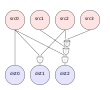
\includegraphics[width=1.0\linewidth]{relest_soc.pdf}
\end{figure}
\end{columns}

\end{frame}
\notepage{
Understanding how your components are interacting boils down to figuring out how
binary data streams are interacting.
As hardware engineers that means we browse through waveforms looking for things
which might be related.
This means that we end up with very long parallel streams of binary data
and the goal is to find how these data sources are connected to each other
with some logical function.
In general once we know that two things are connected, somehow, the exact way in
which they are connected is less interesting.

On this diagram, each node represents a wire such as valid, cache-miss, idle,
etc that we can monitor.
And in real-life there is no distiction between src and dst nodes - that's just
for my convenience in a statistical experiment.
So the goal here is to work out the logical functions between each node.

} % }}}

\begin{frame} \frametitle{Correlation Metrics} % {{{ 0m55s

\begin{align}
\cov(X, Y) &= \sEx{ \left(X-\sEx{X}\right) \left(Y-\sEx{Y}\right) }
    = \sEx{XY} - \sEx{X} \sEx{Y}
\\
\label{eq:covariance_limits}
X,Y \in [0,1] &\implies \frac{-1}{4} \leq \cov(X,Y) \leq \frac{1}{4}
\\
\label{eq:def_Cov}
\sCov{f_x}{f_y} &:= 4\ \Big| \sEx{f_x * f_y} - \sEx{f_x} \sEx{f_y} \Big|
\end{align}

\begin{align}
X \indep Y &\iff \Pr(X) = \Pr(X|Y)
\\
\label{eq:def_Dep}
\sDep{f_x}{f_y} &:=
        \Bigg| \frac{\sEx{f_x | f_y} - \sEx{f_x}}{\sEx{f_x | f_y}} \Bigg|
    = 1 - \frac{\sEx{f_x} \sEx{f_y}} {\sEx{f_x \odot f_y}}
\end{align}

\end{frame}
\notepage{
I've promised Gaj I won't dwell too much on this, but suffice to say, I've done
some statistical experiments to find useful formulas (called metrics) for
measuring correlation (how related two things are).
Cov is based on covariance, and Dep is based on the theory of independence.

From a practical aspect, the double-stroke E can be implemented as a counter,
the odot can be an AND gate, 1-minus and absolute can be with inverters, and
the 4x can be a shift.
So these two metrics are both useful and hardware-friendly.
} % }}}

\begin{frame} \frametitle{More Correlation Metrics} % {{{ 0m30s

\begin{align}
\label{eq:def_Ham}
\sHam{f_x}{f_y} &= 1 - \sEx{\left| f_x - f_y \right|}
\\
\sCls{f_x}{f_y} &= 1 -
    \frac{ \sqrt{\sEx{\left| f_x - f_y \right|^2}} }
         { \sqrt{2} }
\\
\label{eq:def_Cos}
\sCos{f_x}{f_y} &=
    \frac{ \sEx{f_x \odot f_y} }
         { \sqrt{\sEx{f_x^2}} \sqrt{\sEx{f_y^2}} }
\\
\sTmt{f_x}{f_y} &=
    \frac{ \sEx{f_x \odot f_y} }
         { \sEx{f_x} + \sEx{f_y} - \sEx{f_x \odot f_y} }
\end{align}

\begin{itemize}
\item NOTE: Positive results only $\in [0, 1]$
\end{itemize}

\end{frame}
\notepage{
I've also looked at some other metrics, but these are found to be less useful,
and/or they're quite expensive in hardware.

One important point is that all these metrics are normalized, meaning that
0 means X and Y are not related, and 1 means fully related basically the same
thing.
} % }}}

\begin{frame} \frametitle{Correlator Usage} % {{{ 1m00s

\begin{figure}
  \centering
  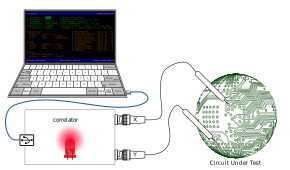
\includegraphics[width=1.0\linewidth]{correlator_usage.pdf}
\end{figure}

\end{frame}
\notepage{
The device I've developed to assist with correlation analysis is called
a correlator.
You get two probes which you stick on to your system at potentially interesting
points, and they're assumed to share a common ground.
Or in a SoC you get two wires and the hardware calculates the metrics quickly.
In Status Monitor terminology that would be two qualifiers which you're trying
to find relationships between which is quite versatile.

The control software can work either interactively for experimenting with
zooming and jitter (which I'll get to in a minute),
or be scripted to record data (typical UltraSoC style).

Just to clarify with a comparison:
Using an oscilloscope or existing Status Monitor, you'd have only one
probe/wire/qualifier that you analyse with voltage-sensor/counter.
Using a correlator you're always doing pairwise analysis.
} % }}}

\begin{frame} \frametitle{Correlator Microarchitecture} % {{{ 1m45s

\begin{figure}
  \centering
  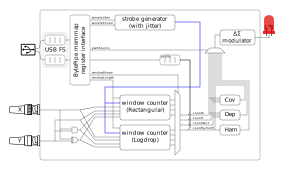
\includegraphics[width=1.0\linewidth]{correlator_uarch.pdf}
\end{figure}

\end{frame}
\notepage{
This is the micro-architecture of a single correlator, without the UltraSoC
integration.
So the BytePipe registers over USB-FS on the left, and fifo in the middle are
swapped out for an UltraSoC messaging system.

As you can see here the central features are the counters which are triggered by
the jittery strobe generator's output in blue.
Each of the counter blocks is actually 4 counters for X, Y, X AND Y, X XOR Y.
And at the end of each time window, a packet containing the upper bits of those
counters is made.

The output LED is driven by a delta-sigma modulator so this can equally be
replaced with an oscilloscope through a low-pass-filter.
An LED is just drawn here because it's more visually intuitive that brighter
means "more correlated".
This is for the case where you've configured the device to use windows so short,
and getting 32b/window, that your datalink can't keep up.
This is a quite acceptable use-case in my opinion, but you have to use
a different tool to see the results, such as passing the delta-sigma signal
through an analog low-pass-filter and recording voltage with a high-speed
oscilloscope.
When you realise that USB-FS (12 Mb/s) maxes out at around 400kB/s, you can see
that isn't very scalable for fast SoCs.
However, the point of my placement here is to get more digital data out through
a USB communicator.
} % }}}

\begin{frame} \frametitle{Timebase (\texttt{windowLength} and \texttt{sampleRate})} % {{{ 1m50s

Balance output data rate with how fast you can detect a change of input
behaviour.

Options for implementation:
\begin{enumerate}
\item IEEE754 floats.
  Easy to understand, trivial to integrate with other systems.
  Costly in area, power, fmax, implementation time.
\item "Standard" counter.
  Simple, small area, low power, high fmax.
  Output requires scaling.
\item Rectangular counter.
  Similar size, power, and fmax as standard counter.
  Output always appears on the same bits, no scaling required.
\end{enumerate}

Correlator moves on exponential scales with
$\texttt{windowLength} = 2^{[3, 16]}$,
$\texttt{sampleRate} = \frac{\SI{48}{\mega\hertz}}{2^{[0, 15]}}$.


\end{frame}
\notepage{
In correlation analysis you have to define how often you take samples on the
probes and how many samples are in a window, just like fourier analysis.
Using these windows you can calculate, using metrics, various definitions of
correlation between two bit-streams.
You can actually use the metrics to analyse normalized data, i.e anything
expressible as a percentage not exceeding 100, not just bitstreams, but my
research hasn't looked at any demonstrations of that type of data.

Floating point hardware is a rabbit hole I don't wish to disappear into, so I'm
using fixed point arithmetic with integer counters.
I use the term "standard" counter here because I use something a little
different.
On a standard counter like in a status monitor, you always accumulate from the
lower bits, then read back the full result.

What I do is define a result size, say 8b, which comes from a larger, say 32b
counter.
On a standard counter, when you want to read the 8 MSb of your result you need
to work out what bitrange that is, depending on how long your counter has been
running (window-length).
} % }}}

\begin{frame} \frametitle{Rectangular Counter} % {{{ 1m15s

\begin{figure}
  \centering
  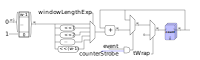
\includegraphics[width=1.0\linewidth]{corrCountRect.pdf}
\end{figure}

\end{frame}
\notepage{
Hopefully this diagram makes it a bit clearer.
windowLengthExp is as register which defines the length of the window as a power
of 2.

If windowLengthExp is set to its maximum, then the counter always increments by
1, like a standard counter.
You want to interactively experiment like fiddling with knobs on an
oscilloscope, the counter increments by different powers of 2.
As a consequence, your result MSb always appears in the top bits of count.

Now you're probably thinking this is quite a convoluted way to save some
bandwidth, and it's not that hard to do the calculation at the end of a window
- which is absolutely correct.
The usefulness of this scaling-increment approach comes out when you want to use
a non-rectangular window function.
} % }}}

\begin{frame} \frametitle{Windowing (\texttt{windowShape})} % {{{ 1m25s

Modelling attention/focus or performing Fourier analysis necessitates some sort
of bell curve.

Options for implementation:
\begin{enumerate}
\item Pre-computed coefficient table, indexed by $t$, with a multiplier.
  The usual method, flexible with window shapes,
  almost arbitrary frequency response.
  Requires significant memory and supporting peripheral circuitry.
\item Logdrop counter.
  No memory required, only a small number of gates/\gls{LUT}s.
  Fixed frequency response.
\end{enumerate}

Correlator selects \texttt{windowShape} as either Rectangular or Logdrop.

\end{frame}
\notepage{
You want to use a bell-curve sort of window function to "focus" analysis on
a particular region of time, without harsh discontinuities at the edges of that
region.
This is standard practice for Fourier/frequency analyses.

The usual method of applying a window function is to have a big ROM with
pre-computed coefficients and you just need a memory as big as your longest
supported window.
The problem is that can be quite a lot of memory, especially when you think
very long windows, say 2-to-the-32 cycles which is about 4-and-a-half seconds at
1GHz.

Of course, you can get around this by having some circuitry to calculate
on-the-fly, but that's getting a bit complex and likely expensive in hw for
things like a CORDIC pipeline to calculate sines and logarithms.
I wanted a window function which could calculate coefficients on the fly, so not
using any memory, and be very cheap/simple in hw.
} % }}}

\begin{frame} \frametitle{Logdrop Window Function} % {{{ 1m50s

\begin{align}
t \in \integers \ [0, N); \quad N = 2^p; \quad p \in \integers > 2
\\
\label{eq:def_logdrop}
w[n] = 2^{\lceil\log_2\min(n+1, N-n)\rceil - \log_2\frac{N}{2}}
  \quad \in \reals \cap (0, 1]
\end{align}

\begin{columns}[T]
\column{0.50\textwidth}
\centering
\begin{figure}
    \includegraphics[width=0.99\linewidth]{logdropWindow_0idx_N32.pdf}
\end{figure}
~
\column{0.50\textwidth}
\centering
\begin{figure}
    \includegraphics[width=0.99\linewidth]{logdropWindow_freq_N32.pdf}
\end{figure}
\end{columns}

\end{frame}
\notepage{
The window function I'm proposing I've called "logdrop" because it drops off in
logarithmic steps.
As you can see, the center-half of the time window has a coefficient of 1, like
full attention, and less attention is paid to the regions near the beginning and
end.

All coefficients in a window function are between 0 and 1 inclusive so this
means the counter must be able to increment by less than 1.
This is where the scaling-increment counter approach comes into play.
To do that you define an accumlation precision of, say 16b where all bits set
corresponds to 1, and all but the upper corresponds to 0.5.

While the equation defining the time-domain coefficients may look complex at
first, I can promise it reduces down to a very small number of gates/LUTs.
Of course, synth results depend on the application, but it indicates ballpark
figures are quite low.
On Lattice iCE40, a fairly low-spec FPGA family, using a precision of 16b, and
a counter of a futher 16b this synthezises to around 50 LUT4s.
} % }}}

\begin{frame} \frametitle{Logdrop Window Function (N=64k)} % {{{ 0m50s

\begin{columns}[T]
\column{0.50\textwidth}
\centering
\begin{figure}
    \includegraphics[width=0.99\linewidth]{logdropWindow_0idx_N64k.pdf}
\end{figure}
~
\column{0.50\textwidth}
\centering
\begin{figure}
    \includegraphics[width=0.99\linewidth]{logdropWindow_freq_N64k.pdf}
\end{figure}
\end{columns}

\end{frame}
\notepage{
A nice property of this window function is that the frequency response changes
as you change the window length.
That's nice because it fits intuitively with how confident we are in the
results.
I.E. With a longer window, we have more data, and can expect less "noise", seen
as harmonic spikes, in our results.
That's quite similar to harmonic noise in Fourier analysis.

In the previous slide the window length was 32, and in this slide the window
length is 64k.
As you can see, the main lobe protrudes higher and the side-lobes become
smoother.
} % }}}

\begin{frame} \frametitle{Logdrop Counter} % {{{ 0m30s

\begin{figure}
  \centering
  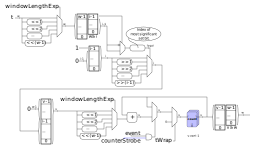
\includegraphics[width=1.0\linewidth]{corrCountLogdrop.pdf}
\end{figure}

\end{frame}
\notepage{
Coming back to the logical topology of a counter which changes its accumulation
amount depending on position in a time window, you can see that it's very
similar to the "rectangular" counter.
And again, the 8b result appears in the top few bits of count at the end of the
window.
} % }}}

\begin{frame} \frametitle{Relations with delays (\texttt{sampleJitter})} % {{{ 1m25s

Relationship may have a delay of some cycles.

Options for implementation:
\begin{enumerate}
\item Buffer both X and Y, then compute relationships for all values of delay.
  All results available for all data.
  Extremely resource intensive, both compute and memory.
\item Randomized testing with jittery sample clock.
  Can detect relationships within a range of delay values with small amount of
  resource, and that range may be very large.
  Requires searching in real-time to pick out exact delay values.
\end{enumerate}

Correlator selects \texttt{sampleJitter} variance $\frac{2^{[0, 8]}-1}{256}$.

\end{frame}
\notepage{
Moving on to a different sub-problem, is that of delay between signals.
It would be great if we didn't have clock domains and everything was
equivalent to single-cycle like in the quantum photonics world.
But for us silicon folk we have to deal with delays.

For example, X is "CPU5 started executing function foo" and Y is "L3 cache-miss",
we're going to have a bit of a delay between the two signals, possibly 100s of
cycles.
In case it isn't obvious, doing a cycle-by-cycle comparison of two bit vectors
for hundreds of offset shifts is not a feasible hardware solution!
And transferring cycle-by-cycle values off-chip at full rate isn't very scalable
either, so a different approach is required.
} % }}}

\begin{frame} \frametitle{Sampling Strobe} % {{{ 1m40s

\begin{align}
\label{eq:strobePeriodApproxPDF}
\Pr(\text{period is $n$ cycles}) &\approx
  \frac{1}{\sqrt{sj}\sqrt{2\pi}} {\exp}{\left( -\frac{1}{2} \left( \frac{n-s}{\sqrt{sj}} \right)^2 \right)}
\end{align}

\begin{columns}[T]
\column{0.50\textwidth}
\centering
\begin{figure}
    \includegraphics[width=0.99\linewidth]{strobePeriodApproxPDF.pdf}
\end{figure}
~
\column{0.50\textwidth}
\centering
\begin{figure}
    \includegraphics[width=0.99\linewidth]{strobe_design.pdf}
\end{figure}
\end{columns}

\end{frame}
\notepage{
Instead we can take a statistical approach.
This assumes we can get a clock faster than the signals change, so in our
example we'd probably want "CPU5 *is* executing foo" and "L3 *is* fetching"
rather than single cycle pulses.

For a statistical approach to taking samples we need something that can take
a sample *approximately* every n cycles rather than *exactly*, and be able to
control how approximate the sampler is.
Fortunately, using a slightly odd counter with a small PRNG on the side, we can
make a strobe with a Gaussian-distributed period.
In this example, a sample is taken every *approximately* 100 cycles; sometimes
99, sometimes 102, but averaging out at 100.

Three variances are shown in this picture, but the ctrlJitter signal is just an
integer going into a comparator, so it's cheap to use whatever variance you
want.
In my implementation I'm providing 8 variances, all powers of two, just because
I can save some register bits.
As the 8 variances are in a logarithmic scale, the peaks of these PDFs are
vertically equally spaced.

So by analysing samples which are taken irregularly, we can find some
correlation between things like X and Y-delayed-by a few cycles.
Then you can adjust the variance to narrow down the delay, and if you have
a configurable-length buffer on the inputs you can find an exact inter-signal
delay.
} % }}}

\begin{frame} \frametitle{Outputting results (\texttt{ledSource})} % {{{ 0m20s

Options for output:
\begin{enumerate}
\item Exact values for all results over data link.
  Allows arbitrary offline processing.
  May require too much bandwidth and storage.
\item Approximate value for results as fast as humans can consume in real-time.
  View result as brightness of an LED.
  Good for interactive searching but not offline processing.
\end{enumerate}

Correlator selects \texttt{ledSource} to be one of $\Cov$, $\Dep$, or $\Ham$.
The first two because they are demonstrably useful for the general case, and the
last because it's trivial and may be useful for specific cases.

\end{frame}
\notepage{
I've already mentioned the LED can be used for getting realtime results out at
analog datarate, and though that is supported in the demonstrator integration,
it's not the main point of this placement work.

The LED glows brighter when X and Y are more correlated because the combination
of LED physics and our eye's biology act as a low-pass-filter.
} % }}}

\begin{frame} \frametitle{Correlator Metrics} % {{{ 0m20s

\begin{figure}
  \centering
  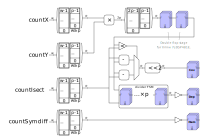
\includegraphics[width=1.0\linewidth]{correlator_metrics.pdf}
\end{figure}

\end{frame}
\notepage{
For the analog output to function it needs to implement the metric calculations
on-chip so this just shows the logical topology, which is quite
hardware-friendly if you don't mind waiting a few cycles for the divider.
} % }}}

\begin{frame} \frametitle{Visualizing Correlation Example} % {{{ 2m15s

\begin{figure}
  \centering
  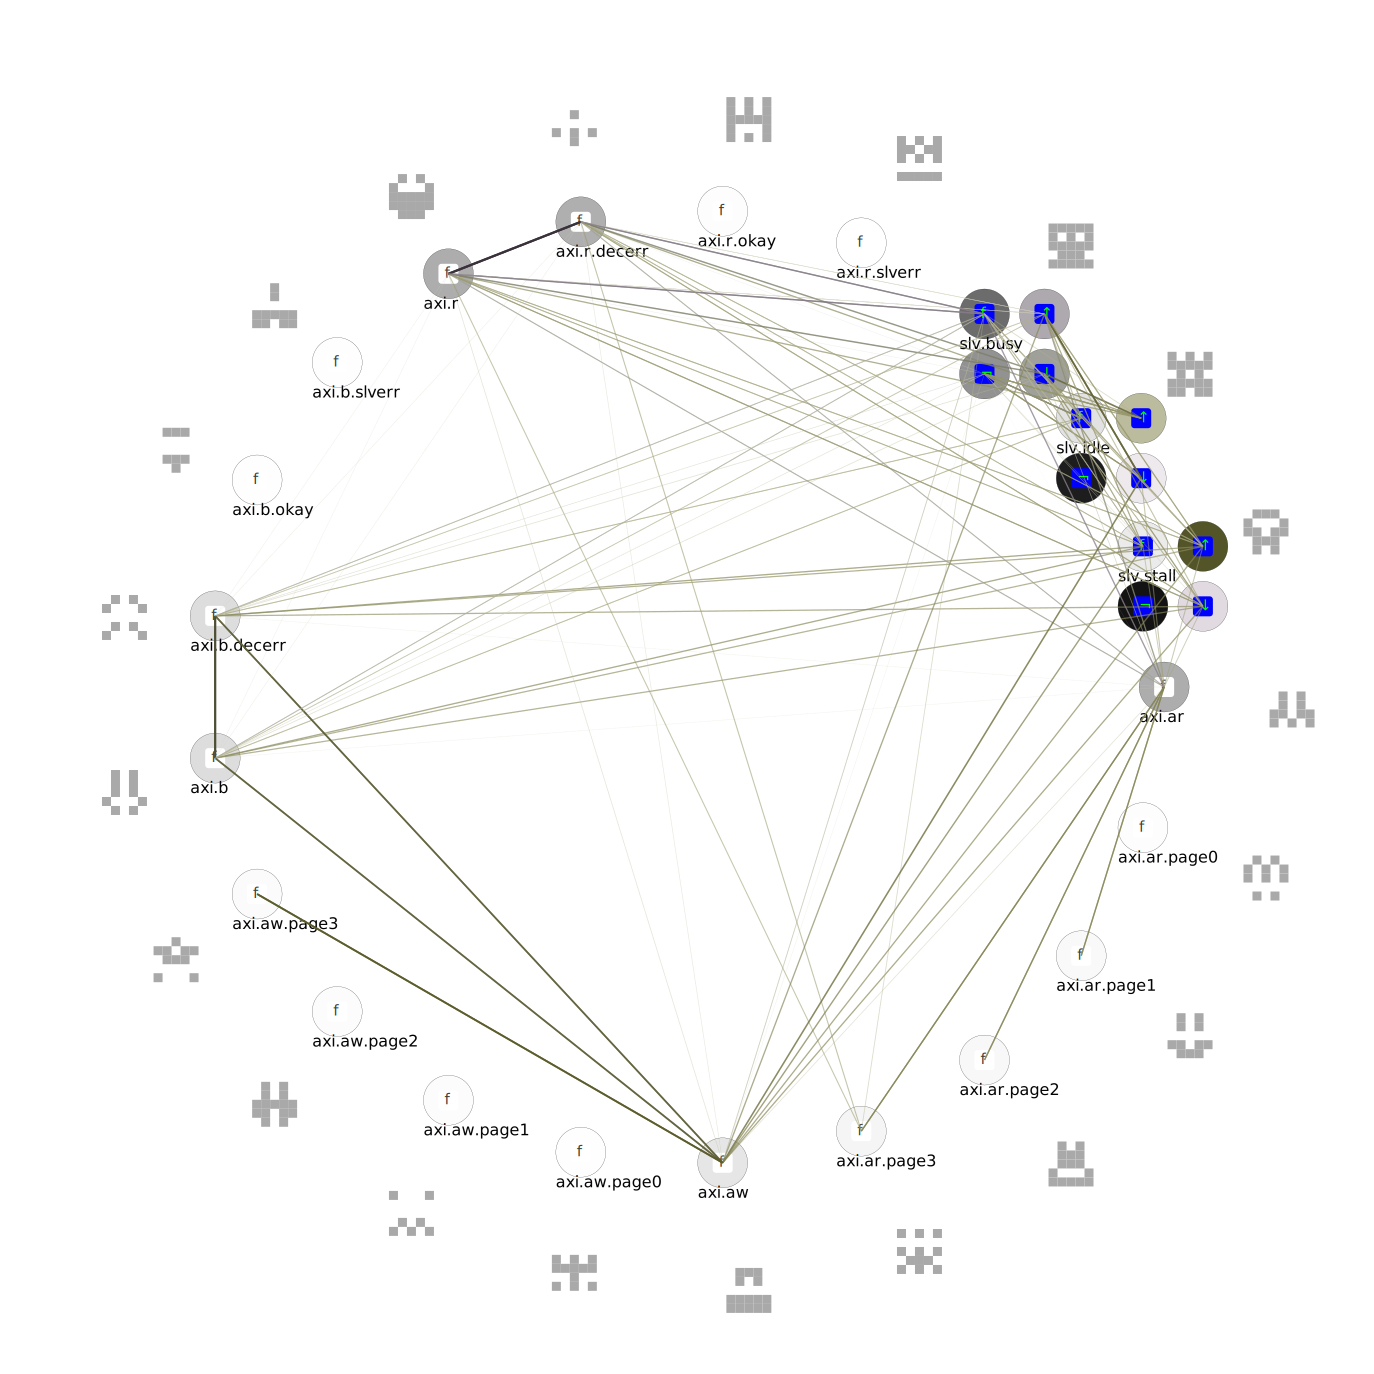
\includegraphics[width=0.7\linewidth]{evaNetgraph_praxi_CovDep_u6144_w512.pdf}
\end{figure}

\end{frame}
\notepage{
Once you have all your data recorded safely off chip and you can calculate
pairwise correlations, what do you do with the results?
I'm not covering it in this presentation but a chapter of my thesis is about
creating intuitive visualizations similar to this.

This diagram shows correlation results for a single time window.
Each node in the circle is a monitored signal and darker lines between them mean
they're more correlated.
There are a few other features to these images like how to determine what color
the lines are, and what different colors mean.

You can then identify densly connected clusters as closely related signals, like
the busy and idle on the top, or the AXI read/write channel interactions in the
middle and bottom.
It's a bit difficult to show in a slide, but as you move through time by moving
to the next image, you can see behavior "signatures" which are easily
recognisable.

So, using the correlator hardware to calculate correlations on a
window-by-window basis, and some diagrams like these, I hope to speed up
debugging some of the difficult high-level system optimization problems we see
as engineers working on silicon and the lowest levels of software.
} % }}}

\begin{frame} \frametitle{Summary} % {{{ 1m15s

\begin{itemize}
\item Assist SoC development via correlation analysis using low-cost hardware.
\item Proof-of-concept integration to UltraSoC Status Monitor.
\item Full details in the thesis (soon).
\end{itemize}

\end{frame}
\notepage{
Let's summarize what's been covered:
What the problem I'm trying to solve is:

Assist in correlation analysis for SoC development.
The device created calculates various metrics of correlation in realtime using
a variety of hardware-friendly techniques including a resource-efficient
windowing function, and a pseudo-random sample strobe.

This device is being integrated into the UltraSoC Status Monitor as a result of
this 1-month placement.
However, the integration is very much a proof-of-concept rather than a
customer-ready product.

For full details you'll have to read the thesis in a couple of months.
My mother can atest it's a great cure for insomnia.
} % }}}

\begin{frame} \frametitle{Questions} % {{{ 0m00s


\end{frame}
\notepage{

} % }}}

\end{document}

